%%
%% This is file `tikzposter-template.tex',
%% generated with the docstrip utility.
%%
%% The original source files were:
%%
%% tikzposter.dtx  (with options: `tikzposter-template.tex')
%%
%% This is a generated file.
%%
%% Copyright (C) 2014 by Pascal Richter, Elena Botoeva, Richard Barnard, and Dirk Surmann
%%
%% This file may be distributed and/or modified under the
%% conditions of the LaTeX Project Public License, either
%% version 2.0 of this license or (at your option) any later
%% version. The latest version of this license is in:
%%
%% http://www.latex-project.org/lppl.txt
%%
%% and version 2.0 or later is part of all distributions of
%% LaTeX version 2013/12/01 or later.
%%


\documentclass{tikzposter} %Options for format can be included here

\usepackage{todonotes}

\usepackage[tikz]{bclogo}
\usepackage{lipsum}
\usepackage{amsmath}

\usepackage{booktabs}
\usepackage{longtable}
\usepackage[absolute]{textpos}
\usepackage[it]{subfigure}
\usepackage{graphicx}
\usepackage{cmbright}
%\usepackage[default]{cantarell}
%\usepackage{avant}
%\usepackage[math]{iwona}
\usepackage[math]{kurier}
\usepackage[T1]{fontenc}
\usepackage{graphicx}

%% add your packages here
\usepackage{hyperref}
% for random text
\usepackage{lipsum}
\usepackage[english]{babel}
\usepackage[pangram]{blindtext}

\colorlet{backgroundcolor}{blue!10}

 % Title, Author, Institute
\title{Tweet Sentiment Extraction}
\author{Jia Huang}
\institute{$^1$ Xi'an Shiyou University, China \\
}
%\titlegraphic{logos/tulip-logo.eps}

%Choose Layout
\usetheme{Wave}

%\definebackgroundstyle{samplebackgroundstyle}{
%\draw[inner sep=0pt, line width=0pt, color=red, fill=backgroundcolor!30!black]
%(bottomleft) rectangle (topright);
%}
%
%\colorlet{backgroundcolor}{blue!10}

\begin{document}


\colorlet{blocktitlebgcolor}{blue!23}

 % Title block with title, author, logo, etc.
\maketitle

\begin{columns}
 % FIRST column
\column{0.5}% Width set relative to text width

%%%%%%%%%% -------------------------------------------------------------------- %%%%%%%%%%
 %\block{Main Objectives}{
%  	      	\begin{enumerate}
%  	      	\item Formalise research problem by extending \emph{outlying aspects mining}
%  	      	\item Proposed \emph{GOAM} algorithm is to solve research problem
%  	      	\item Utilise pruning strategies to reduce time complexity
%  	      	\end{enumerate}
%%  	      \end{minipage}
%}
%%%%%%%%%% -------------------------------------------------------------------- %%%%%%%%%%


%%%%%%%%%% -------------------------------------------------------------------- %%%%%%%%%%
\block{Introduction}{
  With all of the tweets circulating every second it is hard 
  to tell whether the sentiment behind a specific tweet will 
  impact a company, or a person's, brand for being viral
   (positive), or devastate profit because it strikes a negative 
   tone. Capturing sentiment in language is important in these
    times where decisions and reactions are created and updated in 
    seconds. But, which words actually lead to the sentiment
     description? In this competition you will need to pick out
      the part of the tweet (word or phrase) that reflects the 
      sentiment.
  
  	\begin{description}
    \item[The Dataset]  The data set includes three files: the training set, the data set, and the sample set provided.
  	
    \item[Data Format] Each row contains text, a tweet, 
    and a sentiment tag.In the training set, you extract a word or phrase 
    from the tweet (selected\_text) that contains the emotion provided.
    \item[Predicted Results]You are trying to predict words or phrases from the tweets to illustrate the emotions offered.A word or phrase should include 
    all characters in the range (that is, including commas, Spaces, etc.).
  	\end{description}


}
%%%%%%%%%% -------------------------------------------------------------------- %%%%%%%%%%


%%%%%%%%%% -------------------------------------------------------------------- %%%%%%%%%%
\block{The Dataset}{
  There are 27481 pieces of data in the training set,
   among which one piece of data is invalid and shall be deleted.
\begin{itemize}
    %\emph{Group Outlying Aspects Mining}

    \item
    \emph{TextID - The unique ID of each text segment.}
    \item
    \emph{ Text - Tweets.}
    \item 
    \emph{ Sentiment - General sentiment of a tweet.}
    \item 
    \emph{  Selected\_text -(only trains) text that supports the sentiment of the tweet.}
  \end{itemize}
}
%%%%%%%%%% -------------------------------------------------------------------- %%%%%%%%%%


%%%%%%%%%% -------------------------------------------------------------------- %%%%%%%%%%

%\note{Note with default behavior}

%\note[targetoffsetx=12cm, targetoffsety=-1cm, angle=20, rotate=25]
%{Note \\ offset and rotated}

 % First column - second block


%%%%%%%%%% -------------------------------------------------------------------- %%%%%%%%%%
\block{Exploratory Data Analysis}{
  We can see that across the entire dataset, there are 111,117 tweets for 
  neutral emotions, 8,582 tweets for positive emotions, and 7,781 tweets
   for negative emotions.
  \\
 \vspace{.5cm}
  \centering
  \begin{tabular}{ c | c  }
    \toprule
      Nature        & 11117    \\
    \toprule
  positive            & 8582 \\
    \toprule
  negative            &7781    \\
    \bottomrule
\end{tabular}
\vspace{.2cm}
  \begin{description}
  
    \item[Jaccard similarity between Text and selected\_text.]
    As can be seen from the above output results,such as I`d have responded, if I 
    were going,This kind of words has the highest similarity with his
     emotional polarity, with a similarity value of 1, followed by words 
     like leave me alone, with a negative emotional polarity, with a 
     similarity value of 0.6.
     \\
    \item Nuclear distribution graph.
    \\
    
    \begin{center}
      \begin{minipage}{0.5\linewidth}
      \centering
      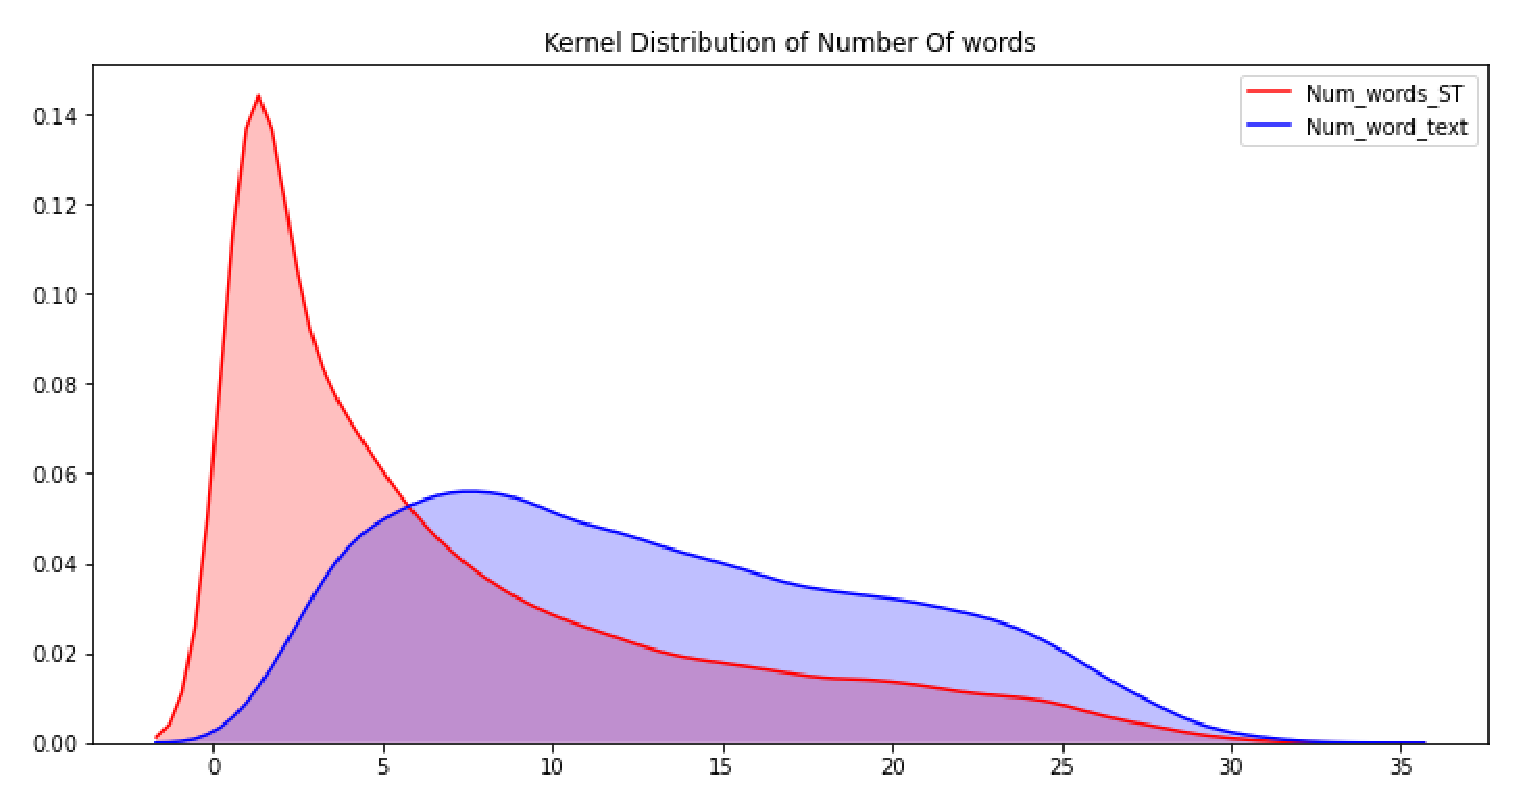
\includegraphics[width=0.9\textwidth]{kaggle/1.1.eps}
      {\small{Flag.1}}
      \end{minipage}
      \hfill
      \\
    \end{center}
    \begin{center}
      \begin{minipage}{0.5\linewidth}
      \centering
      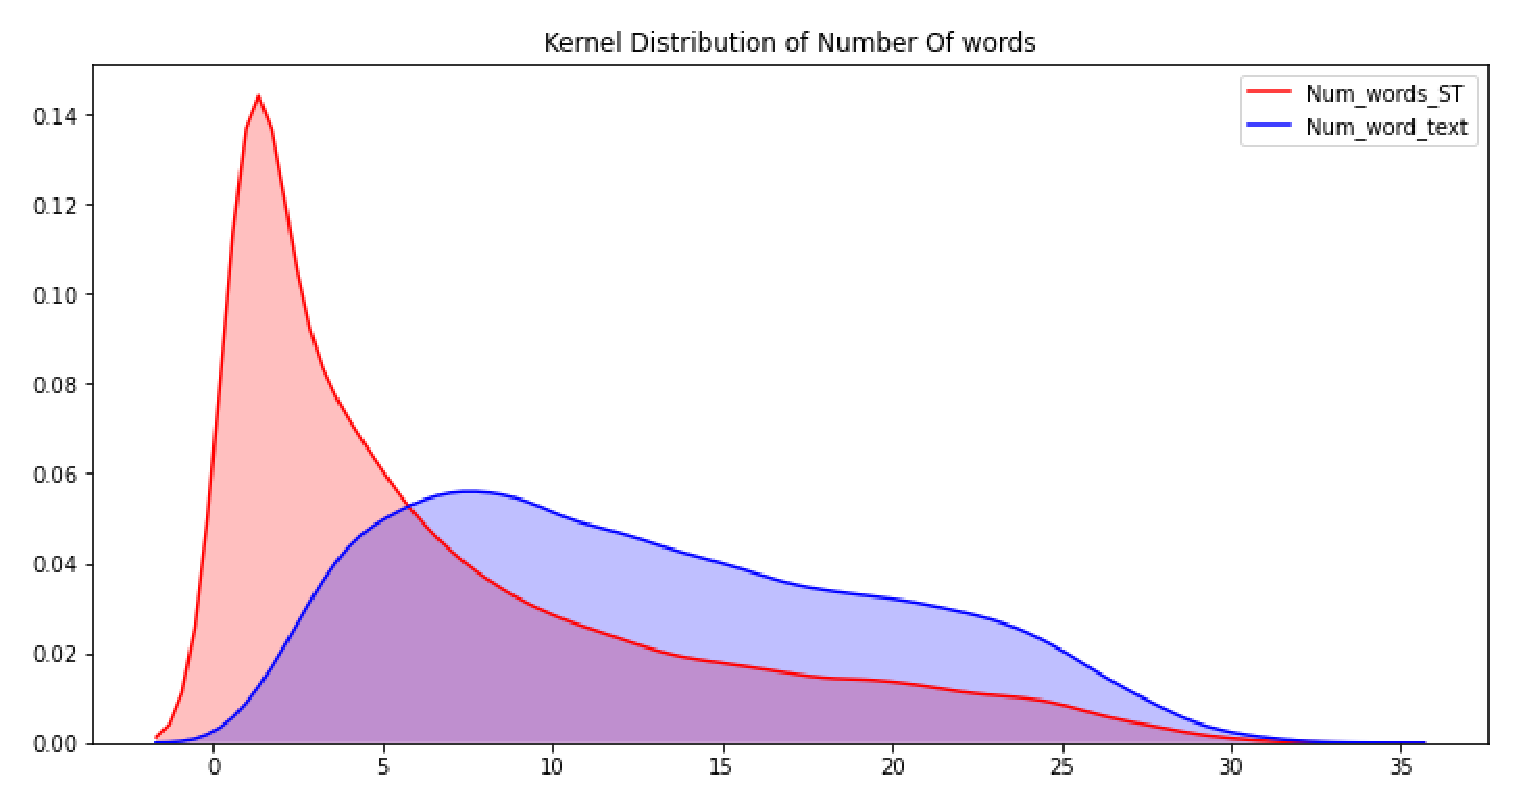
\includegraphics[width=0.9\textwidth]{kaggle/1.2.eps}
      {\small{Flag.2}}
      \end{minipage}
      \hfill
      \\
    \end{center}
  \end{description}
 
  	
%    1) Group Feature Extraction,
%    2) Outlying Degree Scoring, and
%    3) Outlying Aspects Identification.
		
}
%%%%%%%%%% -------------------------------------------------------------------- %%%%%%%%%%


% SECOND column
\column{0.5}
 %Second column with first block's top edge aligned with with previous column's top.

%%%%%%%%%% -------------------------------------------------------------------- %%%%%%%%%%
\block{Exploratory Data Analysis}{
  \begin{center}
    \begin{minipage}{0.5\linewidth}
    \centering
    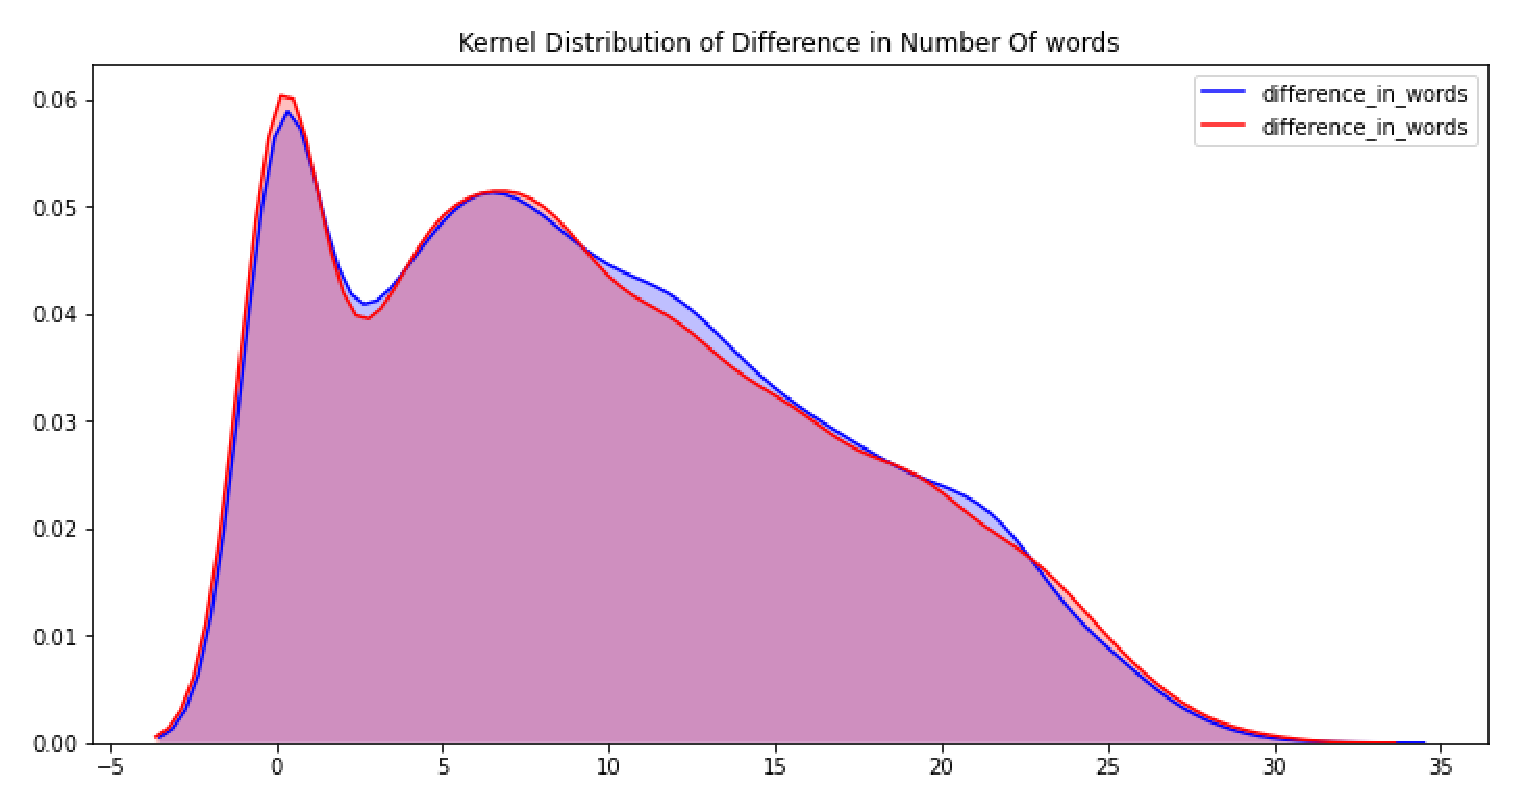
\includegraphics[width=0.9\textwidth]{kaggle/1.3.eps}
    {\small{Flag.3}}
    \end{minipage}
    \hfill
    \\
  \end{center}
  ~\\
  ~\\
  As can be seen from the above figure, the Jaccard similarity of positive or negative text
   and selected\_text has two sharp kurtosis around 1.0 or 0.1.The word 
   length difference also has two kurtosis, where the difference of 0 is
    a sharp kurtosis.That means that a large percentage of positive or
     negative text is the same as selected\_text.
~\\
It's also possible to use the word cloud to show how often words appear in different categories of Twitter.
~\\
The three word clouds show the most frequently used words in tweets
for each of the three E-polarities.
For example, we can clearly see that we usually use words like happy, 
good and so on to express our happy mood, and these words are also 
obvious in our output word cloud.
\begin{tikzfigure}%[Overall architecture of \emph{GOAM} algorithm]
    \missingfigure[figcolor=white]{Testing figcolor}
\end{tikzfigure}
}
%%%%%%%%%% -------------------------------------------------------------------- %%%%%%%%%%
% Second column - first block


%%%%%%%%%% -------------------------------------------------------------------- %%%%%%%%%%
\block[titleleft]{Model Construction and Training.}
{
  Model for training in the large-scale corpus, it concluded that the
   word vector can be used in different field of NLP, but all of these 
   training requires a lot of GPU, for the average person is unable to
   model parameters, used after fine-tuning in our NLP tasks.Here I used 
   Huggingface's open source Transformers library, which provides a lot of 
   directly called and built using PyTorch or TensorFlow.
\vspace{.5cm}
\begin{itemize}
  \item Divide the training set into 5 copies, and take 4 copies of training and 1 copy for verification.
  \item Three epochs are trained each time, and parameters of the epoch with the lowest Loss in verification set are taken.We get a new model at the end of each training session, so we end up with 5 models.
  \item When making predictions, the prediction results of these five models will be averaged.
  \item The predicted values of the five trained models were averaged.
\end{itemize}
\vspace{.2cm}



\vspace{.5cm}     
\begin{minipage}{0.5\linewidth}
    \centering
    \begin{tikzfigure}
    \missingfigure[figcolor=white]{Testing figcolor}

    {\small{New Orleans Pelicans on FT\%}}
    \end{tikzfigure}%
\end{minipage}
\hfill
\begin{minipage}{0.5\linewidth}
    \centering
    \begin{tikzfigure}
    \missingfigure[figcolor=white]{Testing figcolor}

    {\small{New Orleans Pelicans on FTA}}
    \end{tikzfigure}%
\end{minipage}
\vspace{.2cm}
}
%%%%%%%%%% -------------------------------------------------------------------- %%%%%%%%%%


% Second column - second block
%%%%%%%%%% -------------------------------------------------------------------- %%%%%%%%%%
\block[titlewidthscale=1, bodywidthscale=1]
{Conclusion}
{
    Through this project, we further understand the related contents of
 big data analysis, and also have a preliminary understanding of natural
  language processing. I believe this project experience will be of 
  great help in the following study.

}
%%%%%%%%%% -------------------------------------------------------------------- %%%%%%%%%%


% Bottomblock
%%%%%%%%%% -------------------------------------------------------------------- %%%%%%%%%%
\colorlet{notebgcolor}{blue!20}
\colorlet{notefrcolor}{blue!20}
\note[targetoffsetx=8cm, targetoffsety=-4cm, angle=30, rotate=15,
radius=2cm, width=.26\textwidth]{
Acknowledgement
\begin{itemize}
    \item
    International Cooperation Project (Y7Z0511101)
    of IIE,
    Chinese Academy of Sciences
 \end{itemize}
}

%\note[targetoffsetx=8cm, targetoffsety=-10cm,rotate=0,angle=180,radius=8cm,width=.46\textwidth,innersep=.1cm]{
%Acknowledgement
%}

%\block[titlewidthscale=0.9, bodywidthscale=0.9]
%{Acknowledgement}{
%}
%%%%%%%%%% -------------------------------------------------------------------- %%%%%%%%%%

\end{columns}


%%%%%%%%%% -------------------------------------------------------------------- %%%%%%%%%%
%[titleleft, titleoffsetx=2em, titleoffsety=1em, bodyoffsetx=2em,%
%roundedcorners=10, linewidth=0mm, titlewidthscale=0.7,%
%bodywidthscale=0.9, titlecenter]

%\colorlet{noteframecolor}{blue!20}
\colorlet{notebgcolor}{blue!20}
\colorlet{notefrcolor}{blue!20}
\note[targetoffsetx=-13cm, targetoffsety=-12cm,rotate=0,angle=180,radius=8cm,width=.96\textwidth,innersep=.4cm]
{
\begin{minipage}{0.3\linewidth}
\centering

\includegraphics[width=24cm]{logos/tulip-wordmark.eps}
\end{minipage}
\begin{minipage}{0.7\linewidth}
{ \centering
 The $11^{th}$ International Conference on Knowledge Science,
  Engineering and Management (KSEM 2018),
  17-19/08/2018, Changchun, China
}
\end{minipage}
}
%%%%%%%%%% -------------------------------------------------------------------- %%%%%%%%%%


\end{document}

%\endinput
%%
%% End of file `tikzposter-template.tex'.
